\section{Training Details}
\label{sec:appendix_training}

Table~\ref{tab:hyperparams} lists the full hyperparameter configurations for both recovery stages described in Section~\ref{sec:exp_setup}. All four pruning criteria share identical SFT and GRPO settings; the only difference is Random's shorter generation limit, inherited from the TRL library default.

\begin{table}[h]
\centering
\small
\caption{Hyperparameter details for SFT warmup and GRPO recovery stages. All methods share the same GRPO configuration; Random uses the TRL default generation limit (marked with $^\dagger$).}
\label{tab:hyperparams}
\resizebox{\columnwidth}{!}{%
\begin{tabular}{@{}lll@{}}
\toprule
Parameter & SFT & GRPO \\
\midrule
Learning rate & $2 \times 10^{-5}$ & $1 \times 10^{-6}$ \\
Batch size & 1 & 1 \\
Gradient accumulation & 8 & 1 \\
Max sequence length & 2{,}048 & -- \\
Max new tokens & -- & 1{,}024\,$^\dagger$512 \\
Optimizer & AdamW & AdamW \\
Epochs / Steps & 2 epochs & 100 steps \\
KL coefficient $\beta$ & -- & 0.01 \\
Sampling temperature & -- & 0.4 \\
Num generations per prompt & -- & 8 \\
Reward & -- & Binary (exact match) \\
Loss formulation & Cross-entropy & DAPO-style clipped \\
\texttt{reward\_desert\_patience} & -- & 50 \\
\bottomrule
\multicolumn{3}{l}{\footnotesize $^\dagger$Random uses TRL default of 512 tokens; all other methods use 1{,}024.} \\
\end{tabular}}
\end{table}

\section{Algorithm}
\label{sec:appendix_algo}

Algorithm~\ref{alg:rasp} summarizes the complete pruning comparison procedure from Section~\ref{sec:method}: shared structural analysis (importance and CKA overlap computation), criterion-specific scoring (Eqs.~\ref{eq:standard}--\ref{eq:cka_only}), and two-stage recovery (SFT warmup followed by GRPO).

\begin{algorithm}[h]
\caption{Controlled Pruning Comparison Framework}
\label{alg:rasp}
\begin{algorithmic}[1]
\Require Model $\mathcal{M}$, calibration data $\mathcal{D}_\text{cal}$, target sparsity $s$, scoring criterion $\mathcal{C} \in \{\text{Std}, \text{RASP}, \text{CKA}, \text{Rand}\}$, layer floor $\tau$
\Ensure Pruned and recovered model $\mathcal{M}'$
\Statex \textit{\% Stage 1: Shared Structural Analysis}
\For{each structure $h \in \mathcal{H}$}
    \State Compute importance $I(h)$ via Eq.~\eqref{eq:importance}
    \State Collect activations $\mathbf{X}_h$ on $\mathcal{D}_\text{cal}$
\EndFor
\For{each layer $\ell = 1, \ldots, L$}
    \For{each structure $h_i$ in layer $\ell$}
        \State $F(h_i) \gets \frac{1}{|\mathcal{H}_\ell|-1} \sum_{j \neq i} \text{CKA}(\mathbf{X}_{h_i}, \mathbf{X}_{h_j})$
    \EndFor
\EndFor
\Statex \textit{\% Stage 2: Criterion-Specific Scoring}
\For{each structure $h \in \mathcal{H}$}
    \State $S(h) \gets \mathcal{C}(I(h), F(h))$ \hfill $\triangleright$ Eq.~\ref{eq:standard}, \ref{eq:score}, \ref{eq:cka_only}, or random
\EndFor
\State Sort $\mathcal{H}$ by $S(h)$ ascending; prune lowest up to $s$, subject to $\tau$
\Statex \textit{\% Stage 3: Two-Stage Recovery}
\State $\mathcal{M}_\text{warm} \gets \text{SFT}(\mathcal{M}_\text{pruned}, \mathcal{D}_\text{sft})$ \hfill $\triangleright$ restore EOS \& format
\State $\mathcal{M}' \gets \text{GRPO}(\mathcal{M}_\text{warm}, \mathcal{D}_\text{rlvr})$ \hfill $\triangleright$ recover reasoning
\State \Return $\mathcal{M}'$
\end{algorithmic}
\end{algorithm}

\section{Inference Efficiency}
\label{sec:appendix_inference}

\begin{table}[h]
\centering
\small
\caption{Inference characteristics at 20\% sparsity (single-GPU, no contention). Pruning reduces parameters by 19\% and memory by ${\sim}$28\%, with TTFT improving 18\%. Per-token throughput decreases 19\% (0.81$\times$) due to non-uniform layer widths from full-layer removal that current GPU kernels do not optimize.}
\label{tab:inference}
\resizebox{\columnwidth}{!}{%
\begin{tabular}{@{}lcccc@{}}
\toprule
Configuration & TPS\,(tok/s) & TTFT\,(ms) & Per-token\,(ms) & Params\,(B) \\
\midrule
Dense 7B & 72.0 & 20.1 & 13.9 & 7.62 \\
CKA-only 20\% & 58.3 & 16.4 & 16.7 & 6.16 \\
Standard 20\% & 58.2 & 16.4 & 16.7 & 6.16 \\
\bottomrule
\end{tabular}}
\end{table}

All pruned models achieve ${\sim}$28\% memory reduction from structural parameter removal.
TTFT (time to first token) improves by 18\% (20.1$\to$16.4\,ms), reflecting faster prefill with fewer parameters.
Per-token throughput decreases by 19\% (72.0$\to$58.3 tok/s, or 13.9$\to$16.7\,ms per token), consistent with non-uniform layer widths creating computational bottlenecks that current GPU kernels do not optimize away.
CKA-only and Standard show identical throughput (58.3 vs 58.2 tok/s), confirming that the pruning criterion affects recovery capacity but not inference speed at matched sparsity.

\section{CKA Coefficient $\alpha$ Ablation}
\label{sec:appendix_alpha}

\begin{table}[t]
\centering
\small
\caption{Dose-response analysis: effect of CKA coefficient $\alpha$ on GSM8K accuracy ($N{=}1{,}319$) at 20\% MLP channel sparsity. $\alpha{=}0$ reduces to Standard (importance-only); higher $\alpha$ weights representational diversity. Best in \textbf{bold}.}
\label{tab:alpha}
\begin{tabular}{@{}cccc@{}}
\toprule
$\alpha$ & SFT Acc.\,(\%) & GRPO Acc.\,(\%) & $\Delta$\,(pp) \\
\midrule
0.5 & 60.73 & 61.18 & $+$0.45 \\
1.0 & 61.49 & 60.88 & $-$0.61 \\
\textbf{2.0} & \textbf{64.97} & \textbf{66.11} & $+$1.14 \\
3.0 & 64.14 & 63.46 & $-$0.68 \\
4.0 & 61.94 & 62.77 & $+$0.83 \\
\bottomrule
\end{tabular}
\end{table}


On GSM8K, the dose-response curve across $\alpha \in \{0.5, 1.0, 2.0, 3.0, 4.0\}$ reveals an inverted-U pattern peaking at $\alpha{=}2.0$ (SFT 64.97\%, GRPO 66.11\%, $\Delta{=}{+}1.14$\,pp; Table~\ref{tab:alpha}).
At $\alpha{=}0.5$, importance still dominates; recovery is low (SFT 60.73\%, GRPO 61.18\%).
At $\alpha{=}1.0$ (\rasp{}), GRPO collapses (peak reward 0.061, accuracy 60.88\%, $\Delta{=}{-}0.61$\,pp).
$\alpha{=}3.0$ (SFT 64.14\%, GRPO 63.46\%, $\Delta{=}{-}0.68$\,pp) excludes a plateau hypothesis: accuracy drops 2.65\,pp from the $\alpha{=}2.0$ peak, confirming that the optimum is a true peak rather than a saturation regime.
At $\alpha{=}4.0$, CKA overlap dominates; the model recovers to 62.77\% GRPO accuracy (SFT 61.94\%, $\Delta{=}{+}0.83$\,pp) with active GRPO learning (reward 0.146$\to$0.256$\to$0.198).
Reward-accuracy decoupling holds at every $\alpha$ value: $|\Delta| \leq 1.14$\,pp across all five points.

\section{Extended Training Dynamics}
\label{sec:appendix_extended}

To test whether importance-dominated criteria simply need more training to overcome collapse (\S\ref{sec:extended_analysis}), we extend GRPO from 100 to 300 steps for CKA-only and Standard (Figure~\ref{fig:extended_training}).
At 300 steps, GSM8K accuracy remains unchanged: CKA-only 64.37\% (identical to the 100-step seed 42 result), Standard 59.29\% (within the 100-step seed variance of $\pm$0.38\,pp).
CKA-only reward rises from 0.354 (peak at step 100) to 0.308 (step 300), yet accuracy does not improve, directly confirming reward-accuracy decoupling at this training horizon.
Standard reward remains flat (0.054--0.058) with $f_0 > 0.5$ throughout, confirming that additional training does not resolve the structural collapse identified in Section~\ref{sec:recovery_gradient}.

\section{MATH-500 Out-of-Distribution Evaluation}
\label{sec:appendix_math500}

\begin{table}[h]
\centering
\small
\caption{MATH-500 out-of-distribution evaluation ($N{=}500$, greedy decoding, \texttt{max\_new\_tokens=2048}). CKA-only and Standard both outperform \rasp{} and Random; the CKA-only--Standard GRPO gap is 0.6\,pp (vs.\ 4.6\,pp on GSM8K), consistent with difficulty and truncation compressing scores toward a floor. Best per section in \textbf{bold}.}
\label{tab:math500}
\begin{tabular}{@{}lccc@{}}
\toprule
Method & SFT\,(\%) & GRPO\,(\%) & $\Delta$\,(pp) \\
\midrule
Dense & \multicolumn{3}{c}{53.0\,$^\dagger$} \\
\midrule
\multicolumn{4}{l}{\textit{20\% sparsity --- method comparison}} \\
CKA-only & \textbf{27.4} & \textbf{27.6} & $+$0.2 \\
Standard & 25.6 & 27.0 & $+$1.4 \\
\rasp{} ($\alpha{=}1.0$) & 21.6 & 23.0 & $+$1.4 \\
Random & 16.6 & 15.0 & $-$1.6 \\
\midrule
\multicolumn{4}{l}{\textit{20\% sparsity --- $\alpha$ dose-response}} \\
$\alpha{=}0.5$ & 26.8 & 26.8 & $+$0.0 \\
$\alpha{=}2.0$ & 25.6 & \textbf{27.4} & $+$1.8 \\
$\alpha{=}3.0$ & 23.6 & -- & -- \\
$\alpha{=}4.0$ & \textbf{27.8} & 27.2 & $-$0.6 \\
\midrule
\multicolumn{4}{l}{\textit{25\% sparsity}} \\
CKA-only & 18.8 & 17.6 & $-$1.2 \\
Standard & 15.4 & -- & -- \\
\bottomrule
\multicolumn{4}{p{0.85\columnwidth}}{\footnotesize $^\dagger$Over half of Dense responses truncated at 2048 tokens (73.6\% at 4096); all pruned models evaluated under the same constraint.}
\end{tabular}
\end{table}


CKA-only and Standard both outperform \rasp{} and Random on MATH-500 (SFT: 27.4\%, 25.6\% vs.\ 21.6\%, 16.6\%; GRPO: 27.6\%, 27.0\% vs.\ 23.0\%, 15.0\%), consistent with GSM8K.
However, the CKA-only--Standard gap narrows substantially: from 4.6\,pp (GSM8K SFT) to 1.8\,pp (MATH-500 SFT) to 0.6\,pp (MATH-500 GRPO).
Middle-ranked methods also swap positions (Standard $>$ \rasp{} on MATH-500 vs.\ \rasp{} $>$ Standard on GSM8K).
This narrowing reflects two compounding factors: MATH-500's higher intrinsic difficulty (the unpruned model achieves only 53.0\% vs.\ 90.83\% on GSM8K) and generation-length truncation at the 2{,}048-token evaluation limit (over half of dense-model responses are truncated; Table~\ref{tab:math500}), both of which compress all pruned methods toward a performance floor and reduce inter-method differentiation (\S\ref{sec:ood}).
CKA-only also produces more efficient reasoning: only 22\% of completions are truncated at the 2{,}048-token limit (mean 655 tokens) versus Standard's 44\% (mean 1{,}128 tokens), indicating that the preserved structure enables shorter reasoning chains rather than longer ones.
The $\alpha$ dose-response effect is not statistically significant on MATH-500: SFT accuracy varies by ${\sim}$8\,pp across $\alpha$ values, but with stderr ${\approx}$2\,pp per point, attributable to high truncation rates at the 2048-token limit and floor effects at this difficulty level.
The inverted-U pattern is validated on GSM8K (Table~\ref{tab:alpha}); MATH-500 does not resolve the dose-response shape.

\section{MBPP Code Generation}
\label{sec:appendix_mbpp}

To test whether reward-accuracy decoupling extends beyond math reasoning (\S\ref{sec:ood}), we evaluate on MBPP~\citep{austin2021mbpp} ($N{=}374$ code-generation problems; Table~\ref{tab:mbpp}).

\begin{table}[h]
\centering
\small
\caption{MBPP code generation accuracy ($N{=}374$, greedy decoding). All fine-grained pruning methods converge near a capability floor (${\sim}$75\% code capability loss vs Dense), limiting differentiation (${\sim}$1\,pp range, within stderr). ShortGPT shows a larger GRPO delta ($+$4.01\,pp) but at the 95\% CI boundary (stderr ${\approx}$1.55\,pp).}
\label{tab:mbpp}
\begin{tabular}{@{}lccc@{}}
\toprule
Method & SFT\,(\%) & GRPO\,(\%) & $\Delta$\,(pp) \\
\midrule
Dense & -- & 53.48 & -- \\
\midrule
CKA-only 20\% & 12.83 & 14.17 & $+$1.34 \\
Standard 20\% & 12.03 & 13.10 & $+$1.07 \\
\rasp{} ($\alpha{=}1.0$) 20\% & 11.76 & 13.10 & $+$1.34 \\
\midrule
ShortGPT 20\%$^\dagger$ & 10.43 & 14.44 & $+$4.01 \\
\bottomrule
\multicolumn{4}{l}{\footnotesize $^\dagger$Depth pruning; removes entire layers.}
\end{tabular}
\end{table}


MBPP GRPO deltas are uniformly slightly positive across all fine-grained methods (mean $+$1.25\,pp), but none are statistically significant at this sample size ($N{=}374$; stderr ${\approx}1.7$\,pp).
This directional consistency may reflect a weak task-specific GRPO effect at the capability floor rather than a violation of reward-accuracy decoupling.

\section{CKA Scoring Stability}
\label{sec:appendix_cka_stability}

Section~\ref{sec:structural_analysis} notes that our intra-layer CKA use avoids known cross-layer sensitivities~\citep{davari2023cka,klabunde_similarity_survey_2023}. Table~\ref{tab:cka_stability} validates ranking stability across calibration set sizes.

\begin{table}[h]
\centering
\small
\caption{CKA scoring stability across calibration sizes. Spearman $\rho$ between structure rankings produced by different calibration set sizes. High correlation ($\rho \geq 0.964$) indicates that CKA-based scoring is robust to calibration data volume.}
\label{tab:cka_stability}
\begin{tabular}{@{}lcc@{}}
\toprule
Calibration Sizes & Spearman $\rho$ (min) & Spearman $\rho$ (mean) \\
\midrule
256 / 512 / 1024 & 0.964 & 0.979 \\
\bottomrule
\end{tabular}
\end{table}


CKA-based structure rankings are highly stable across calibration data volumes: Spearman $\rho$ between rankings from 256, 512, and 1024 calibration samples ranges from 0.964 to 0.979, confirming that the scoring criterion is robust to calibration set size within this range.

\section{Gradient Signal Analysis}
\label{sec:appendix_gradient}

We compare per-layer gradient magnitudes during early GRPO training ($N{=}200$ GSM8K calibration samples) across three pruning criteria using paired Wilcoxon signed-rank tests.

\begin{table}[h]
\centering
\small
\caption{Pairwise gradient magnitude ratios during GRPO training. Ratio: mean gradient magnitude of method A divided by method B across 56 parameter groups (28 layers $\times$ 2 projections). Significant layers: count where paired Wilcoxon signed-rank $p{<}0.05$.}
\label{tab:gradient_flow}
\begin{tabular}{@{}lcc@{}}
\toprule
Comparison & Gradient Ratio & Sig.\ Layers \\
\midrule
CKA-only vs Standard & 2.89$\times$ & 55\,/\,56 \\
CKA-only vs \rasp{} & 2.26$\times$ & 56\,/\,56 \\
\rasp{} vs Standard & 1.28$\times$ & 45\,/\,56 \\
\bottomrule
\end{tabular}
\end{table}

The gradient magnitude hierarchy (CKA-only $\gg$ \rasp{} $>$ Standard) mirrors the recovery capacity hierarchy (GSM8K: 64.39\% $>$ 60.88\% $>$ 59.84\%), with bootstrap 95\% CIs for all ratios excluding 1.0.
This is consistent with diversity preservation enabling stronger training signals during GRPO, though the evidence is correlational: an alternative explanation (that CKA-only retains more functional structure, producing higher initial loss and naturally larger gradients) cannot be ruled out.

\section{Seed Reproducibility}
\label{sec:appendix_seed}

We verify that the recovery capacity spectrum (\S\ref{sec:recovery_gradient}) is robust to GRPO random seed variation.
CKA-only GSM8K accuracy across 3 GRPO seeds: 64.37\% (seed 42), 64.22\% (seed 123), 64.59\% (seed 456), yielding mean 64.39\% $\pm$ 0.19\,pp.
Standard: mean 59.84\% $\pm$ 0.38\,pp across the same 3 seeds.
The 4.55\,pp gap between CKA-only and Standard is stable, with non-overlapping ranges across all seeds.
See Table~\ref{tab:multiseed} for the full breakdown including 15\% sparsity results.

\section{Sparsity Cliff at 30\%}
\label{sec:appendix_sparsity_cliff}

Section~\ref{sec:sparsity_cliff} notes that all methods collapse at 30\% sparsity. Table~\ref{tab:sparsity_cliff} provides the full results.

\begin{table}[t]
\centering
\caption{Sparsity cliff at 30\% structured sparsity. All tested pruning criteria collapse, with near-zero accuracy and EOS generation rates below 6\%.}
\label{tab:sparsity_cliff}
\begin{tabular}{@{}lccc@{}}
\toprule
Method & $N$ & Acc.\,(\%) & EOS Rate\,(\%) \\
\midrule
Standard & 200 & 4 & 5.5 \\
\rasp{} ($\alpha{=}1.0$) & 200 & 0 & 3.0 \\
CKA-only & 500$^\dagger$ & 1.6 & --$^\dagger$ \\
\bottomrule
\multicolumn{4}{@{}l}{\footnotesize $^\dagger$Terminated early after collapse confirmed; 8/500 correct.}
\end{tabular}
\end{table}


All tested methods collapse at 30\% sparsity: Standard retains only 4\% accuracy, CKA-only 1.6\%, and \rasp{} at $\alpha{=}1.0$ drops to 0\%.
This capacity threshold is independent of pruning criterion, validating 20\% as the practical operating point for DeepSeek-R1-Distill-Qwen-7B and confirming that the recovery capacity spectrum (\S\ref{sec:recovery_gradient}) reflects how methods allocate a limited pruning budget rather than absolute capacity differences.

\section{Multi-Seed GRPO Results}
\label{sec:appendix_multiseed}

\begin{table}[h]
\centering
\small
\caption{Multi-seed GRPO results on GSM8K ($N{=}1{,}319$). CKA-only, Standard, and Random each trained with 3 GRPO seeds (42, 123, 456); pruning calibration and SFT are identical across all runs within each sparsity level.}
\label{tab:multiseed}
\begin{tabular}{@{}llccc@{}}
\toprule
Sparsity & Method & Mean Acc.\,(\%) & Std\,(pp) & Seeds \\
\midrule
\multirow{4}{*}{20\%} & CKA-only & 64.39 & 0.19 & 3 \\
 & Standard & 59.84 & 0.38 & 3 \\
 & \rasp{} & 60.88 & -- & 1 \\
 & Random & 50.72 & 0.15 & 3 \\
\midrule
\multirow{2}{*}{15\%} & CKA-only & 72.76 & 0.57 & 3 \\
 & Standard & 65.56 & 0.50 & 3 \\
\bottomrule
\end{tabular}
\end{table}

At 20\% sparsity, the 4.55\,pp gap between CKA-only and Standard is robust across seeds, with non-overlapping ranges (CKA-only: 64.22--64.59\%, Standard: 59.44--60.20\%).
Standard shows a wider observed range across seeds (0.76\,pp vs 0.37\,pp), consistent with borderline-collapse dynamics where small perturbations produce larger outcome variation.
Random (3 seeds: 50.57\%, 50.72\%, 50.87\%; $\sigma{=}0.15$\,pp, observed range 0.30\,pp) converges in a narrow band with SFT accuracy seed-independent at 51.25\%.
All three seeds satisfy GRPO $\leq$ SFT ($\Delta{=}{-}0.68$, $-$0.53, $-$0.38\,pp), confirming that reward-accuracy decoupling is reproducible across seeds even for stagnating methods.
Note: Standard seed 42 was trained from a separately initialized SFT checkpoint (accuracy 59.21\% vs.\ 59.29\% for seeds 123/456; $\Delta = 0.08$\,pp).
At 15\% sparsity, the gap widens to 7.20\,pp (72.76\% vs 65.56\%, $t{\approx}16.4$, $p{<}0.001$), with non-overlapping ranges (CKA-only: 72.10--73.09\%, Standard: 65.13--65.43\%).

\section{Cross-Sparsity Validation}
\label{sec:appendix_cross_sparsity}

\begin{table}[h]
\centering
\small
\caption{Cross-sparsity validation on DeepSeek-R1-Distill-Qwen-7B. GSM8K accuracy ($N{=}1{,}319$) after SFT warmup and GRPO recovery. 15\% and 20\% GRPO values are mean over 3 seeds (see Tables~\ref{tab:decoupling},~\ref{tab:multiseed}). $^\ddagger$Single seed. Mean $|\Delta| \leq 1$\,pp across all conditions.}
\label{tab:cross_sparsity}
\begin{tabular}{@{}llccc@{}}
\toprule
Sparsity & Method & SFT\,(\%) & GRPO\,(\%) & $\Delta$\,(pp) \\
\midrule
\multirow{2}{*}{15\%} & CKA-only & 72.18 & \textbf{72.76{\scriptsize$\pm$0.57}} & $+$0.58 \\
 & Standard & 66.49 & 65.56{\scriptsize$\pm$0.50} & $-$0.93 \\
\midrule
\multirow{2}{*}{20\%} & CKA-only & 63.91 & 64.39 & $+$0.48 \\
 & Standard & 59.29 & 59.84 & $+$0.55 \\
\midrule
\multirow{2}{*}{25\%$^\ddagger$} & CKA-only & 60.12 & 59.59 & $-$0.53 \\
 & Standard & 50.87 & 51.86 & $+$0.99 \\
\midrule
30\% & All & \multicolumn{3}{c}{Collapse ($\leq$4\%; Table~\ref{tab:sparsity_cliff})} \\
\bottomrule
\end{tabular}
\end{table}

At 15\% sparsity (3-seed mean), the CKA-only advantage widens to $+$7.20\,pp (72.76\% vs 65.56\%), compared to $+$4.55\,pp at 20\%.
CKA-only at 15\% (72.76\%) represents the highest mean accuracy across all experimental conditions, retaining 80.1\% of original dense model performance (90.83\%).
At 25\% sparsity (single seed), Standard's SFT accuracy decline accelerates ($-$7.20\,pp from 15\%$\to$20\%, $-$8.42\,pp from 20\%$\to$25\%), while CKA-only's decline decelerates ($-$8.27\,pp then $-$3.79\,pp).
Reward-accuracy decoupling is preserved ($|\Delta| \leq 1$\,pp for both methods) despite Standard's near-zero peak reward (0.008).

\section{Cross-Scale Validation}
\label{sec:appendix_cross_scale}

To test whether the recovery capacity spectrum generalizes beyond the 7B scale (\S\ref{sec:extended_analysis}), we replicate the comparison on DeepSeek-R1-Distill-Qwen-1.5B~\citep{deepseek2025r1} at 20\% MLP sparsity (Table~\ref{tab:cross_scale}).

\begin{table}[h]
\centering
\small
\caption{Cross-scale validation at 20\% sparsity. 7B: DeepSeek-R1-Distill-Qwen-7B (GSM8K mean over 3 seeds for CKA-only and Standard; see Table~\ref{tab:decoupling}). 1.5B: DeepSeek-R1-Distill-Qwen-1.5B (single seed). GSM8K accuracy ($N{=}1{,}319$). 7B reward = peak across 100 GRPO steps (cf.\ Table~\ref{tab:recovery_gradient}); 1.5B reward = mean across training steps.}
\label{tab:cross_scale}
\resizebox{\columnwidth}{!}{%
\begin{tabular}{@{}lcccc@{}}
\toprule
\multirow{2}{*}{Method} & \multicolumn{2}{c}{7B} & \multicolumn{2}{c}{1.5B} \\
\cmidrule(lr){2-3} \cmidrule(lr){4-5}
 & Peak Rew. & GSM8K\,(\%) & Rew. & GSM8K\,(\%) \\
\midrule
CKA-only & \textbf{0.354} & \textbf{64.39} & \textbf{0.238} & \textbf{35.48} \\
Standard & 0.081 & 59.84 & 0.084 & 22.29 \\
\rasp{} ($\alpha{=}1.0$) & 0.061 & 60.88 & 0.099 & 26.16 \\
Random & 0.190 & -- & -- & -- \\
\bottomrule
\end{tabular}}
\end{table}


The three-method ordering is preserved (CKA-only 35.48\% $\gg$ \rasp{} 26.16\% $>$ Standard 22.29\%), consistent with the 7B results (Table~\ref{tab:recovery_gradient}).
Reward-accuracy decoupling also holds at this scale ($|\Delta| < 1$\,pp: CKA-only $-$0.15, Standard $-$0.61\,pp).
The lower absolute accuracy reflects the 1.5B model's weaker baseline (49.81\% dense vs.\ 90.83\% at 7B), but the relative ordering and decoupling pattern are stable.

\section{Cross-Model Validation within Qwen2.5 Family}
\label{sec:appendix_cross_arch}

\begin{table}[h]
\centering
\small
\caption{Cross-model validation on Qwen2.5-Math-7B~\citep{qwen2.5} (same Qwen2.5 architecture family) at 20\% structured sparsity. Accuracy evaluated on GSM8K ($N{=}200$). Post-SFT reports accuracy $\pm$ binomial standard error ($N{=}200$). EOS rate: fraction of generations that produce a valid end-of-sequence token.}
\label{tab:cross_arch}
\resizebox{\columnwidth}{!}{%
\begin{tabular}{@{}lccc@{}}
\toprule
Method & Post-Prune\,(\%) & Post-SFT\,(\%) & EOS Rate\,(\%) \\
\midrule
CKA-only & 1.0 & \textbf{51.50 $\pm$ 3.53} & 27.0 \\
Standard & 18.5 & 21.00 $\pm$ 2.88 & 36.5 \\
\bottomrule
\end{tabular}}
\end{table}

CKA-only pruning causes near-total initial damage on Qwen2.5-Math-7B (1.0\% post-prune accuracy vs Standard's 18.5\%), yet SFT recovers CKA-only to 51.50\% while Standard remains at 21.00\%.
This post-prune accuracy reversal provides strong evidence that recovery capacity is shaped by preserved network structure rather than starting accuracy.
EOS rates remain below 40\% for both methods, indicating that SFT warmup is less effective on this architecture; GRPO validation is deferred to future work.\footnote{Preliminary GRPO evaluation yields 48.60\% (243/500), but 83.8\% of responses were truncated at 2048 tokens, precluding direct comparison with SFT results.}

\section{Structural Overlap Analysis}
\label{sec:appendix_overlap}

CKA-only and Standard pruning produce markedly different removal patterns across the 28 layers of DeepSeek-R1-Distill-Qwen-7B at 20\% sparsity.
CKA-only concentrates pruning in early layers (L0--9 account for 72.5\% of removed MLP groups), preserving nearly all structures in later layers (L16--27).
Standard distributes removals more uniformly, pruning substantial numbers of groups in late layers (L16--18, L22, L25--26).

The methods share only partial overlap in which structures they remove.
65 MLP groups are pruned exclusively by CKA-only (retained by Standard), concentrated in L6--9 and L27; these are structures that gradient importance scores as important but CKA identifies as redundant with neighboring groups.
Conversely, 46+ groups are pruned exclusively by Standard (retained by CKA-only), concentrated in L16--18, L22, and L25--26; these are structures that gradient importance scores as unimportant but CKA identifies as representationally unique.

This pattern is consistent with the layer-wise CKA similarity analysis (Figure~\ref{fig:cka_heatmap}): CKA-only's aggressive early-layer pruning disrupts dense representations (low diagonal CKA, $\mu{=}0.62$) but preserves diverse late-layer pathways, while Standard's uniform pruning maintains dense fidelity ($\mu{=}0.90$) at the cost of removing unique computational pathways in later layers.

\section{KL Divergence During GRPO Training}
\label{sec:appendix_kl}

KL divergence between the evolving policy and the frozen reference model provides a complementary view of the training dynamics reported in Section~\ref{sec:recovery_gradient}.
Figure~\ref{fig:kl_divergence} tracks this divergence across GRPO training for all four pruning criteria.

\begin{figure}[t]
    \centering
    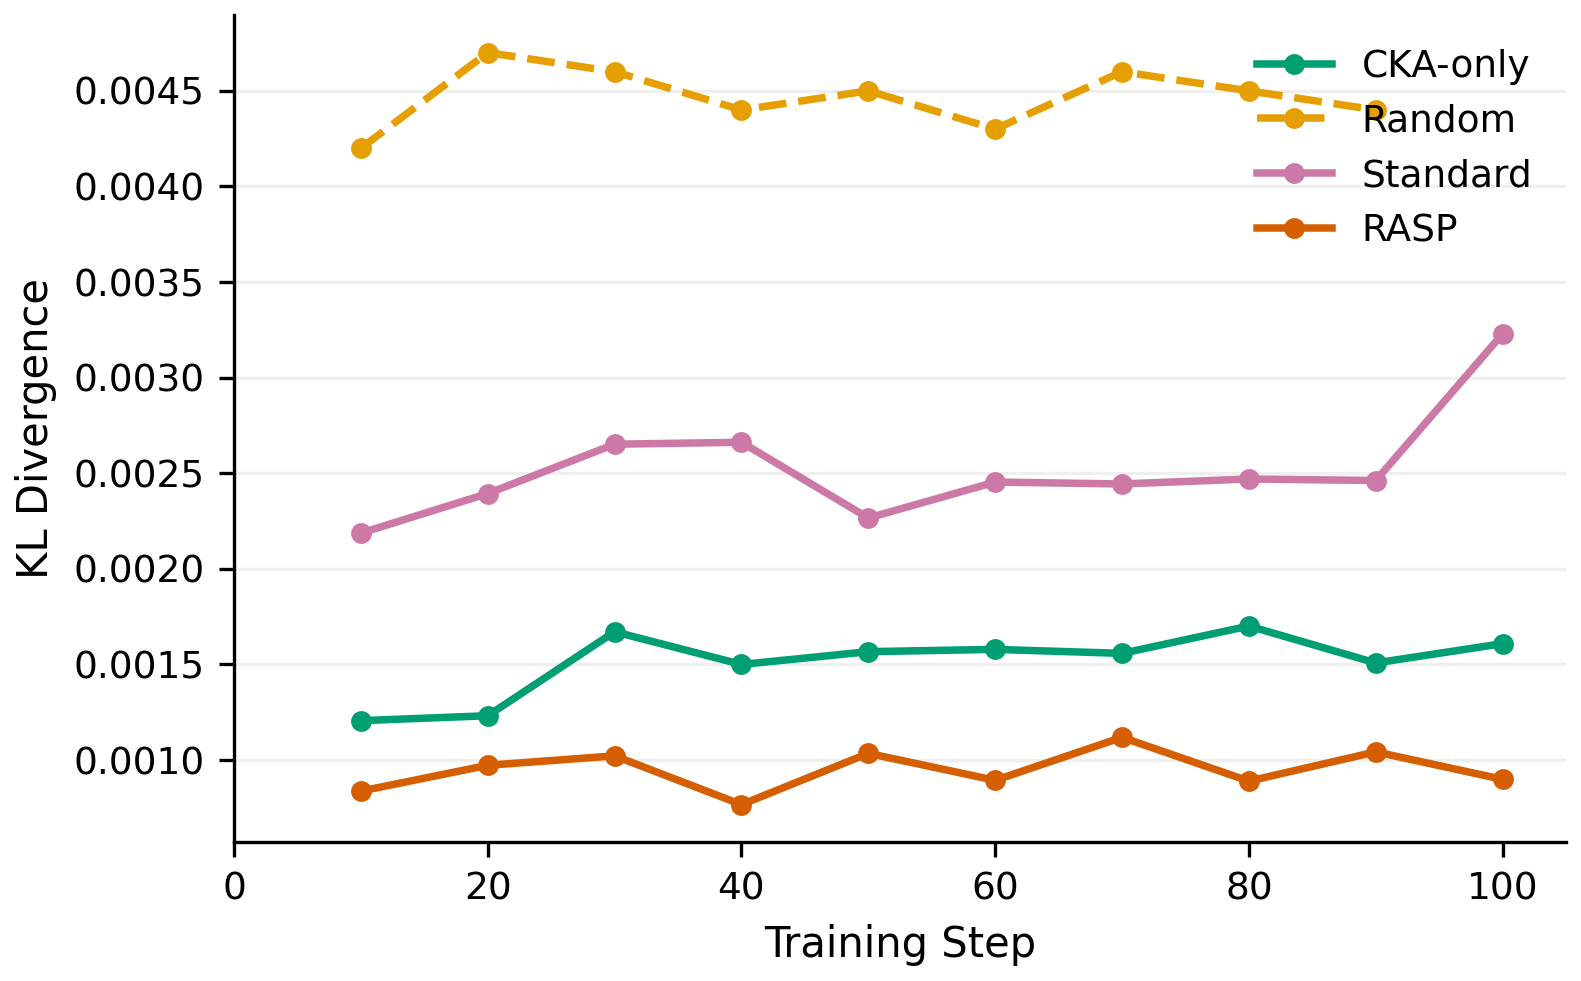
\includegraphics[width=0.75\columnwidth]{figures/paper/fig_appendix_kl.pdf}
    \caption{KL divergence between the policy and reference model during GRPO training. \rasp{} maintains near-zero KL ($<$0.001), consistent with minimal policy movement during collapse. Random shows the highest KL (${\sim}$0.004--0.005), indicating more policy exploration. CKA-only and Standard fall between these extremes.}
    \label{fig:kl_divergence}
\end{figure}

\rasp{} at $\alpha{=}1.0$ maintains near-zero KL ($<$0.001) throughout training, consistent with the reward collapse and vanishing gradients observed in Figure~\ref{fig:training_dynamics}: the policy barely moves from its initialization.
CKA-only and Standard show moderate KL (0.001--0.003), while Random exhibits the highest divergence (${\sim}$0.004--0.005) despite stagnating reward, suggesting undirected exploration without learning.
The KL ordering does not match the recovery capacity spectrum, confirming that policy movement alone does not predict recovery quality.

\section{Depth-First Pruning Baseline}
\label{sec:appendix_depth_first}

CKA-only concentrates pruning in early layers (Section~\ref{sec:extended_analysis}; Appendix~\ref{sec:appendix_overlap}), raising the question of whether its advantage reflects mere depth bias rather than diversity preservation.
As a sanity check, we construct a depth-first baseline: synthetic importance scores force removal of late layers first (L18--27: 0.001, L10--17: 0.5, L0--9: 1.0), then standard pruning at 20\% sparsity.
Both SFT (${\sim}$10\%) and GRPO (${\sim}$8\%) accuracy are near chance (early-stopped at $N{\approx}50$--88 samples due to conclusive results), confirming that naive depth ordering cannot substitute for criterion-based structure selection.
This baseline operates at layer-level granularity (removing entire transformer blocks), unlike CKA-only/Standard/\rasp{} which prune at MLP channel group level; the granularity difference limits direct comparison with our main results and precludes using this baseline as evidence for the recovery capacity spectrum.

\section{Per-Layer Capacity Floor Ablation}
\label{sec:appendix_floor}

\begin{table}[h]
\centering
\small
\caption{Effect of per-layer capacity floor $\tau$ on CKA-only pruning at 20\% sparsity. GSM8K accuracy ($N{=}1{,}319$) after GRPO recovery (100 steps). Default $\tau{=}0.4$.}
\label{tab:floor_ablation}
\begin{tabular}{@{}lcc@{}}
\toprule
Floor $\tau$ & GRPO Acc.\,(\%) & $\Delta$ vs $\tau{=}0.4$\,(pp) \\
\midrule
0.3 & 65.05 & $+$0.68 \\
0.4 (default) & 64.37 & --- \\
0.5 & 61.71 & $-$2.66 \\
0.6 & 62.02 & $-$2.35 \\
\bottomrule
\end{tabular}
\end{table}

The per-layer capacity floor $\tau$ sets the minimum fraction of MLP channel groups retained in each layer, preventing over-pruning of any single layer regardless of its importance score.
We ablate $\tau \in \{0.3, 0.4, 0.5, 0.6\}$ using CKA-only pruning at 20\% sparsity.
Lowering $\tau$ to 0.3 slightly improves accuracy ($+$0.68\,pp), while raising it to 0.5 or 0.6 causes a notable drop ($-$2.66 and $-$2.35\,pp respectively; the difference between 0.5 and 0.6 is not significant at 0.31\,pp $\ll$ stderr $\approx$ 1.3\,pp).
Over-constraining per-layer retention hurts global pruning quality by forcing removal of important structures in unconstrained layers.

\section{TOST Equivalence Testing}
\label{sec:appendix_tost}

To formally assess whether SFT and GRPO produce equivalent GSM8K accuracy, we apply Two One-Sided Tests (TOST) on $N{=}1{,}319$ paired per-example outcomes for CKA-only and Standard at 20\% sparsity across multiple GRPO seeds.
For CKA-only, we include an additional GRPO seed (789) beyond the 3 seeds reported in Table~\ref{tab:multiseed}, yielding 4 paired comparisons; the primary accuracy summary excludes this seed to maintain consistency with the Standard and Random 3-seed protocol.
For each pair, $d_i = \mathbb{1}[\text{SFT correct}]_i - \mathbb{1}[\text{GRPO correct}]_i$, and we test $H_0$: $|\bar{d}| \geq \varepsilon$ against $H_A$: $|\bar{d}| < \varepsilon$.

\begin{table}[h]
\centering
\small
\caption{TOST equivalence results ($\varepsilon{=}2$\,pp). All observed $|\Delta|{<}1$\,pp. $^\dagger$Separate SFT checkpoint (see Appendix~\ref{sec:appendix_multiseed}). $^\ddagger$300-step extended training (Appendix~\ref{sec:appendix_extended}).}
\label{tab:tost}
\begin{tabular}{@{}llrr@{}}
\toprule
Criterion & GRPO variant & $\Delta$ (pp) & $p_\text{TOST}$ \\
\midrule
CKA-only & seed 42 & $-$0.45 & 0.008 \\
CKA-only & seed 123 & $-$0.30 & 0.005 \\
CKA-only & seed 789 & $-$0.15 & 0.001 \\
CKA-only & seed 456 & $-$0.68 & 0.023 \\
\midrule
Standard & seed 123 & $-$0.68 & 0.020 \\
Standard & seed 456 & $-$0.99 & 0.069 \\
Standard & seed 42$^\dagger$ & $-$0.23 & 0.010 \\
Standard & 300-step$^\ddagger$ & $-$0.08 & 0.007 \\
\bottomrule
\end{tabular}
\end{table}

We select $\varepsilon{=}2$\,pp because it is approximately $4\times$ the observed cross-seed standard deviation ($\sigma{=}0.19$\,pp for CKA-only at 20\% sparsity), ensuring the margin reflects meaningful practical differences rather than measurement noise.
At $\varepsilon{=}2$\,pp, 7/8 comparisons reject the null ($p{<}0.05$); the remaining pair (Standard vs.\ seed 456, $\Delta{=}{-}0.99$\,pp) is borderline ($p{=}0.069$).
At $\varepsilon{=}3$\,pp, all 8/8 are significant ($p{<}0.002$).
At $\varepsilon{=}1$\,pp, statistical power is insufficient with binary outcomes at $N{=}1{,}319$.

\section{Discussion}
\label{sec:appendix_discussion}

\paragraph{GRPO as diagnostic probe.}
The decoupling pattern suggests that GRPO may serve as a \emph{diagnostic probe} for pruning quality at moderate sparsity: reward trajectories appear to indicate whether the pruned architecture retains sufficient diversity for RL exploration. This information is not accessible through SFT, which converges to similar accuracy at 20--25\% MLP sparsity.
At 15\% sparsity, GRPO amplifies the CKA-guided advantage ($+$1.51\,pp), suggesting the transition boundary warrants future investigation.

\paragraph{Implications.}
For deployment pipelines that include post-pruning RL, diversity-preserving criteria (CKA-only or high-$\alpha$ \rasp{}) should be preferred.
Our findings complement \citet{selfhealing2025}: while they demonstrate RLVR superiority for unstructured magnitude pruning at 96.5\% retention, within our experimental scope (20--25\% structured MLP sparsity on Qwen2.5-family models), this hierarchy dissolves regardless of pruning criterion. The discrepancy likely reflects differences in experimental setup (pruning granularity, sparsity level) rather than a fundamental property of RL recovery.

\section{Use of AI Assistants}
\label{sec:appendix_ai_assistants}

We used Claude (Anthropic) as an AI coding and writing assistant throughout this work. Specifically:
\begin{itemize}[nosep,leftmargin=*]
    \item \textbf{Code:} drafting experiment scripts, data-processing pipelines, and analysis utilities; debugging and refactoring.
    \item \textbf{Writing:} drafting and revising paper sections, polishing prose, and reformatting \LaTeX{}.
    \item \textbf{Literature:} summarizing related papers to inform the related-work section.
\end{itemize}
